%%%%%%%%%%%%%%%%%%%%%%%%%%%%%%%%%%%%%%%%%
% University Assignment Title Page 
% LaTeX Template
% Version 1.0 (27/12/12)
%
% This template has been downloaded from:
% http://www.LaTeXTemplates.com
%
% Original author:
% WikiBooks (http://en.wikibooks.org/wiki/LaTeX/Title_Creation)
%
% License:
% CC BY-NC-SA 3.0 (http://creativecommons.org/licenses/by-nc-sa/3.0/)
% 
% Instructions for using this template:
% This title page is capable of being compiled as is. This is not useful for 
% including it in another document. To do this, you have two options: 
%
% 1) Copy/paste everything between \begin{document} and \end{document} 
% starting at \begin{titlepage} and paste this into another LaTeX file where you 
% want your title page.
% OR
% 2) Remove everything outside the \begin{titlepage} and \end{titlepage} and 
% move this file to the same directory as the LaTeX file you wish to add it to. 
% Then add \input{./title_page_1.tex} to your LaTeX file where you want your
% title page.
%
%%%%%%%%%%%%%%%%%%%%%%%%%%%%%%%%%%%%%%%%%
%\title{Title page with logo}
%----------------------------------------------------------------------------------------
%	PACKAGES AND OTHER DOCUMENT CONFIGURATIONS
%----------------------------------------------------------------------------------------

\documentclass[12pt]{article}
\usepackage{wrapfig}
\usepackage[english]{babel}
\usepackage[utf8]{inputenc}
\usepackage{amsmath}
\usepackage{graphicx}

\usepackage{float}

\usepackage[colorinlistoftodos]{todonotes}

\begin{document}

\begin{titlepage}

\newcommand{\HRule}{\rule{\linewidth}{0.5mm}} % Defines a new command for the horizontal lines, change thickness here

\center % Center everything on the page
 
%----------------------------------------------------------------------------------------
%	HEADING SECTIONS
%----------------------------------------------------------------------------------------

\textsc{\LARGE Universidad de Sonora }\\[0.3cm] % Name of your university/college
\textsc{\Large Departamento de Ciencias Naturales y Exactas  }\\[0.3cm]
\textsc{\Large Licenciatura en Física }\\[0.3cm]
\textsc{\Large Física computacional I}\\[0.3cm] % Major heading such as course name
 % Minor heading such as course title

%----------------------------------------------------------------------------------------
%	TITLE SECTION
%----------------------------------------------------------------------------------------

\HRule \\[0.1cm]
{ \huge \bfseries Evaluación 2\\  El Atractor de Lorenz, Ejemplo de Caos Dinámico}\\[0.01cm] % Title of your document
\HRule \\[1.5cm]

 
%----------------------------------------------------------------------------------------
%	AUTHOR SECTION
%----------------------------------------------------------------------------------------

\begin{minipage}{0.4\textwidth}
\begin{flushleft} \large
\emph{Alumno:}\\
Gómez García \\Manuel Ignacio\\ %Grupo 1 % Your name
\end{flushleft}
\end{minipage}
~
\begin{minipage}{0.4\textwidth}
\begin{flushright} \large
\emph{Profesor:} \\
Lizarraga Celaya\\Carlos\\%Dept. of CSE % Supervisor's Name
\end{flushright}
\end{minipage}\\[1cm]

% If you don't want a supervisor, uncomment the two lines below and remove the section above
%\Large \emph{Author:}\\
%John \textsc{Smith}\\[3cm] % Your name

%----------------------------------------------------------------------------------------
%	DATE SECTION
%----------------------------------------------------------------------------------------

{\large \date[24 de mayo, 2018 \\Hermosillo, Sonora}\\[1cm] % Date, change the \today to a set date if you want to be precise

%----------------------------------------------------------------------------------------
%	LOGO SECTION
%----------------------------------------------------------------------------------------


\includegraphics[height=5.5cm]{Logo}\\[0.5cm] % Include a department/university logo - this will require the graphicx package
 
%----------------------------------------------------------------------------------------

\vfill % Fill the rest of the page with whitespace

\end{titlepage}

\section{Introducción}
El sistema de Lorenz es un sistema de ecuaciones diferenciales ordinarias estudiadas por Edward Lorenz. La peculiaridad del sistema es que cuenta con soluciones caóticas para ciertos parámetros de sus valores y condiciones iniciales. En particular, el Atractor de Lorenz representa un conjunto de soluciones, las cuales al gráficar generan una figura parecida a una mariposa o al número ocho.

En el año de 1963, Edward Lorenz desarrolló un modelo matemático simplificado para la convección atmosférica. El modelo es un sistema de tres ecuaciones diferenciales ordinarias conocidas como las ecuaciones de Lorenz:

\begin{center}
	$ \dfrac{dx}{dt} = \sigma (y - x) $ \\
    $ \dfrac{dy}{dt} = x (\rho - z) - y $ \\
    $ \dfrac{dz}{dt} = xy - \beta z $
\end{center}

\section{Código en Python}
Representaremos las soluciones del sistema de Lorenz graficamente y para ello hemos hecho uso de la programación  en Python, con esto generaremos diversas gráficas además de aprovechar todas ellas para crear un archivo GIF donde animaremos el trazo de la misma.

\subsection{Atractor de Lorenz: Visualización}
A continuación veremos el código empleado para generar las gráficas y al final mostraremos el producto resultante.

Comenzamos cargando e importando las bibliotecas necesarias dentro de nuestro cuaderno de trabajo.

\begin{figure}[h!]
	\begin{center}
	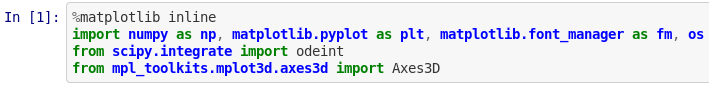
\includegraphics[width=13cm]{Input1V}
    \caption{Importar y cargar bibliotecas.}
    \label{fig1:bibliotecas}
	\end{center}
\end{figure}

Lo siguiente es definir una fuente para las gráficas (esto es opcional), después hemos de crear una carpeta para almacenar los productos generados en caso de que exista.

\begin{figure}[h!]
	\begin{center}
		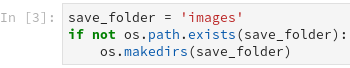
\includegraphics[width=13cm]{Input3V}
        \caption{Carpeta para almacenar productos.}
        \label{fig2:folder}
	\end{center}
\end{figure}

Una vez lista nuestra carpeta $images$ procedemos a definir valores iniciales y parámetros en el código. En este caso es importante tener en cuanto los siguientes valores:

\begin{center}
	$ Sigma ( \sigma ) = 10 $ \\
    $ Rho ( \rho ) = 28 $ \\
    $ Beta ( \beta ) = \dfrac{8}{3} $
\end{center}

\begin{figure}[h!]
	\begin{center}
		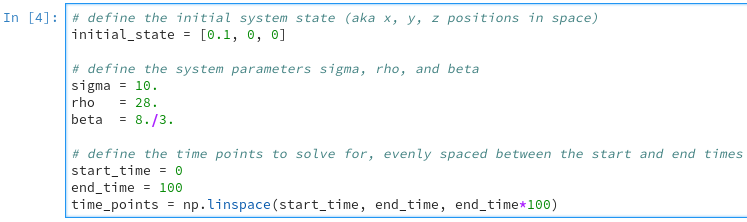
\includegraphics[width=13cm]{Input4V}
        \caption{Definir parámetros y valores iniciales.}
        \label{fig3:Parametros}
	\end{center}
\end{figure}

\vfill
\vline
\space
\par \vspace{2cm}

Ahora debemos de definir/crear las 3 ecuaciones diferenciales ordinarias que conforman las ecuaciones de Lorenz.

\begin{figure}[h!]
	\begin{center}
		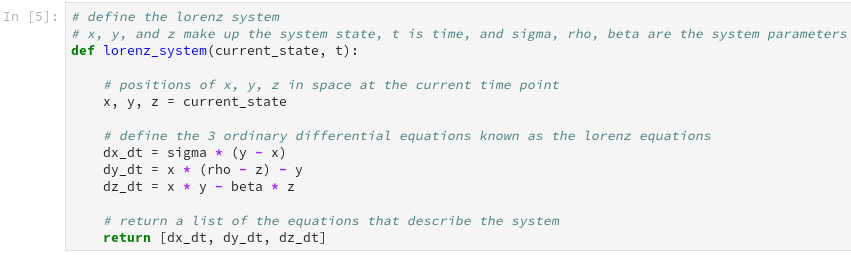
\includegraphics[width=13cm]{Input5V}
        \caption{Definir las ecuaciones de Lorenz.}
        \label{fig4:Lorenz}
	\end{center}
\end{figure}

Una vez que hemos ingresado las ecuaciones en nuestro código es momento de resolverlas y a la vez, de obtener las soluciones en X, Y \& Z.

\begin{figure}[h!]
	\begin{center}
		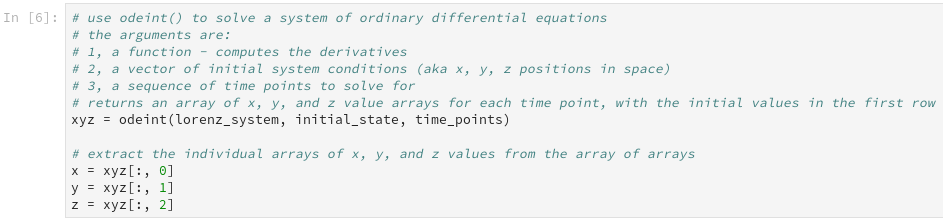
\includegraphics[width=13cm]{Input6V}
        \caption{Resolver el sistema de EDO.}
        \label{fig5:Resolver}
	\end{center}
\end{figure}

\vfill
\vline
\space
\par \vspace{4.5cm}

En este punto, el programa ya ha resuelto el sistema de EDO y simplemente debemos graficarlo en un plano tridimensional, esperando que se genere una imagen parecida a un 8 o una mariposa.

\begin{figure}[h!]
	\begin{center}
		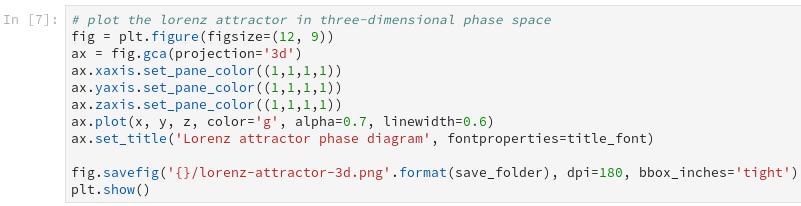
\includegraphics[width=13cm]{Input7V}
        \caption{Generamos la gráfica tridimensional.}
        \label{fig6:Atractor}
	\end{center}
\end{figure}

\begin{figure}[h!]
	\begin{center}
		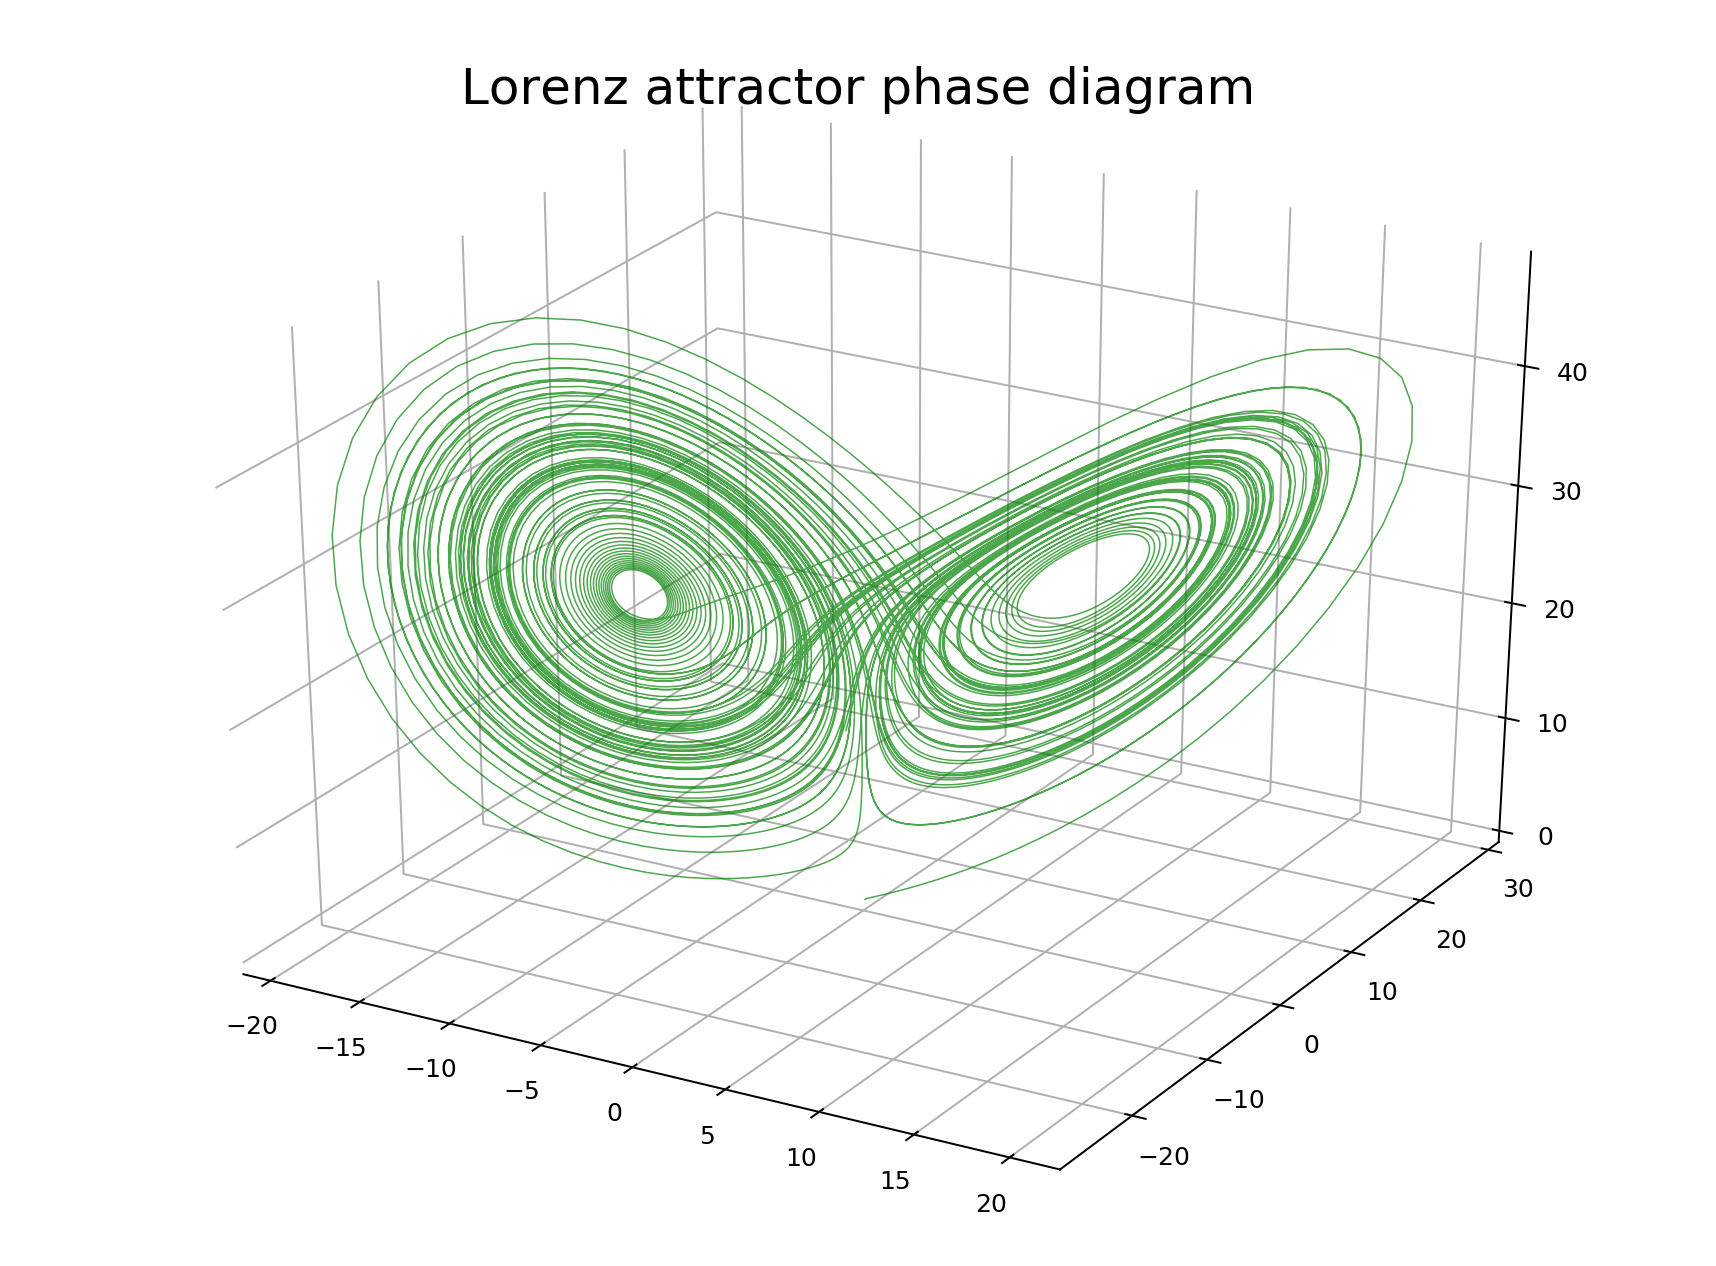
\includegraphics[width=13cm]{AtractorLorenz3D-1}
        \caption{Atractor de Lorenz generado mediante el código.}
        \label{fig7:GrafAtractor}
	\end{center}
\end{figure}

Además, debemos generar una imagen donde se aprecia la gráfica para los planos XY, XZ \& YZ. El código es el siguiente:

\begin{figure}[h!]
	\begin{center}
		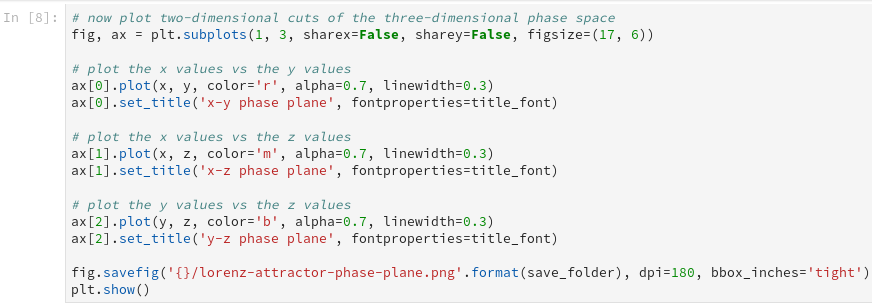
\includegraphics[width=13cm]{Input8V}
        \caption{Generamos una gráfica para cada par de ejes.}
        \label{fig8:AtractorEjes}
	\end{center}
\end{figure}

\begin{figure}[h!]
	\begin{center}
		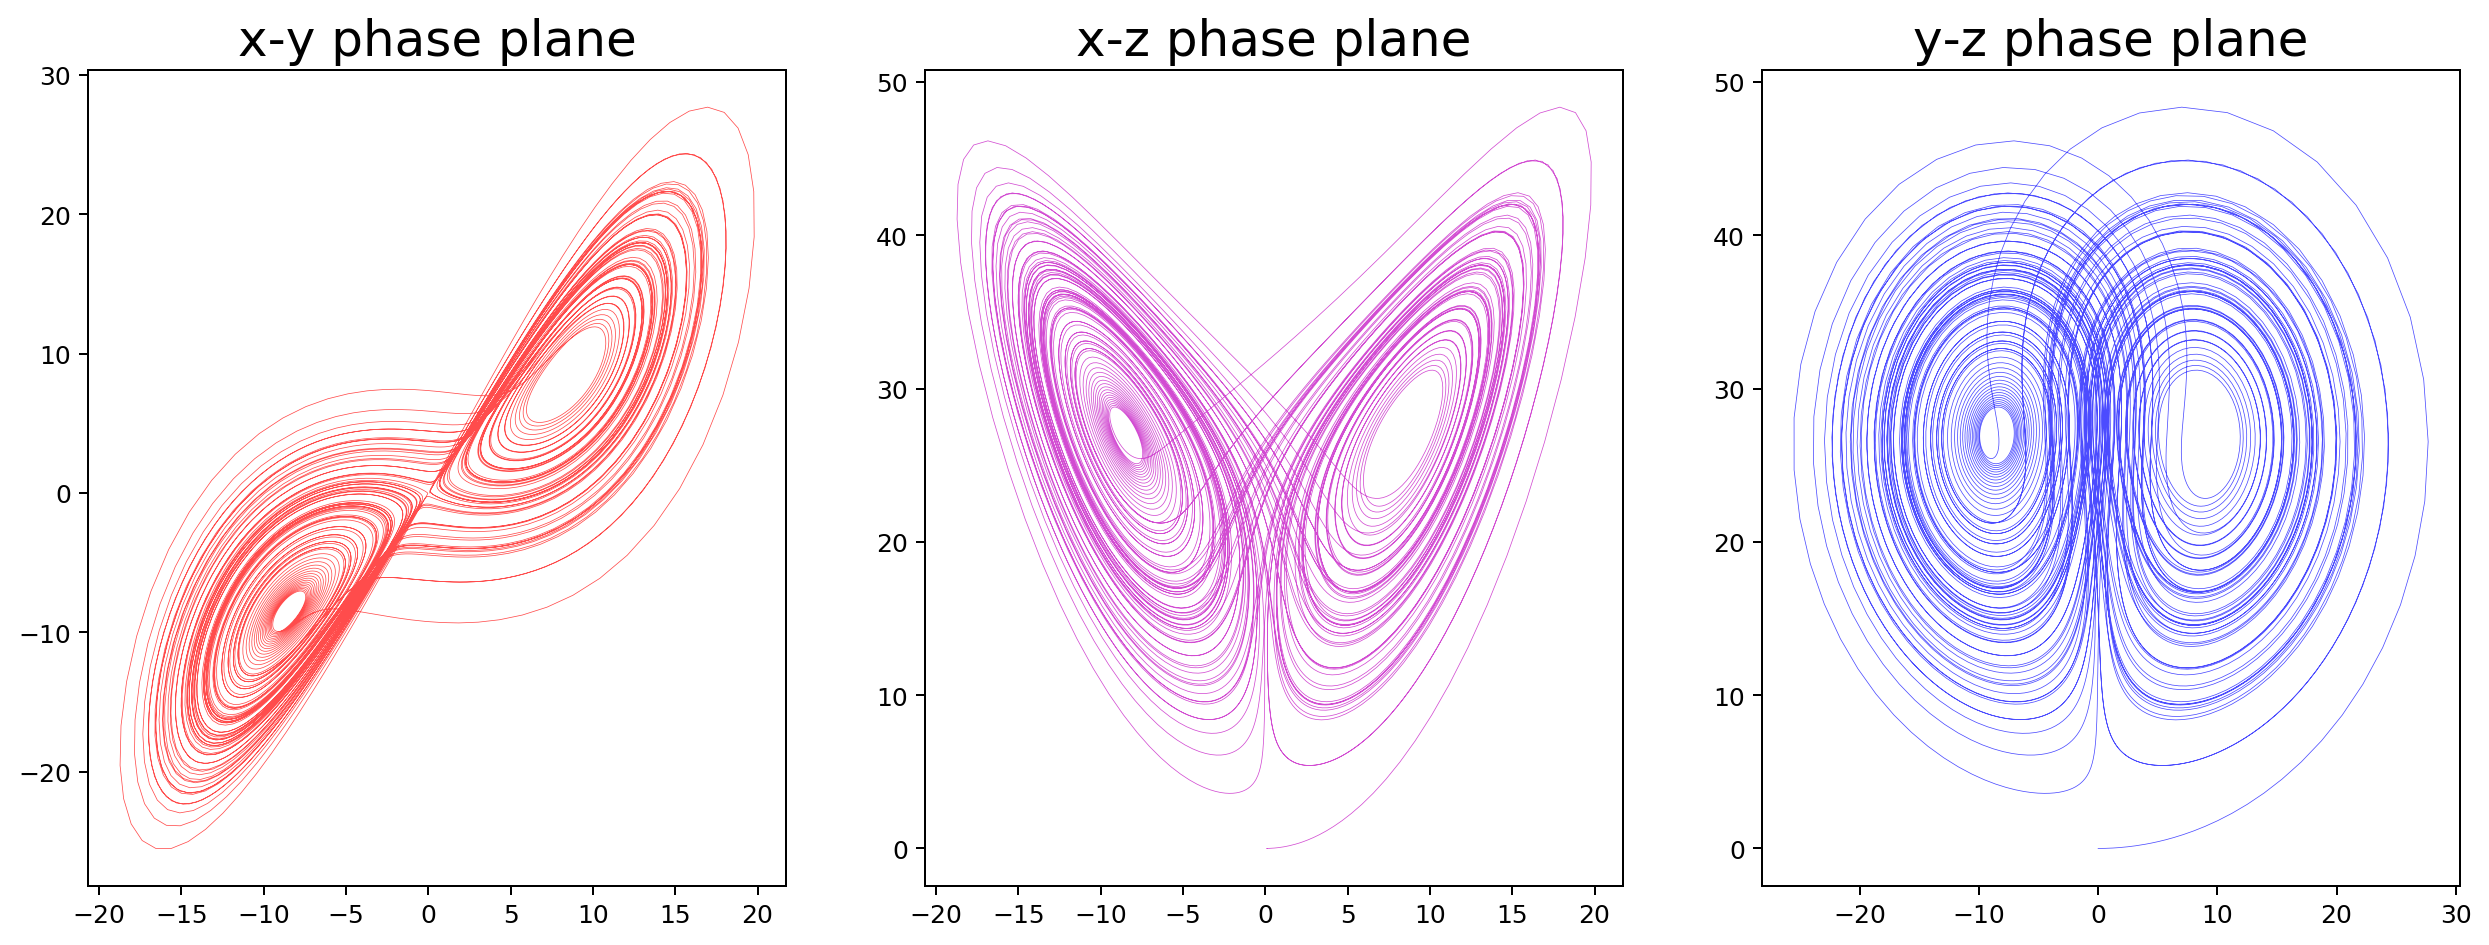
\includegraphics[width=13cm]{AtractorLorenzXYZ-1}
        \caption{Gráficas correspondientes a los ejes.}
        \label{fig9:GrafAtractorEjes}
	\end{center}
\end{figure}

Listo, hemos terminado el código para la visualización de las ecuaciones de Lorenz y obtenido sus soluciones gráficamente.

\vfill
\vline
\space
\par \vspace{2cm}

\subsection{Atractor de Lorenz: Animación}
En esta sección mostraremos el código empleado para la creación de una animación (en este caso un GIF) que muestre la evolución con respecto al tiempo de la solución a las ecuaciones de Lorenz, así como veremos una imagen del producto final.

Como es habitual, comenzamos cargando las bibliotecas a usar en esta ocasión, las cuales son las mostradas en el código a continuación.

\begin{figure}[h!]
	\begin{center}
		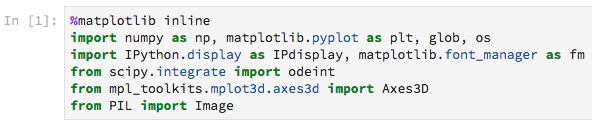
\includegraphics[width=11cm]{Input1A}
        \caption{Bibliotecas necesarias para la animación.}
        \label{fig10:BibliotecasA}
	\end{center}
\end{figure}

De igual manera que en el código de \textsl{Visualización} el segundo bloque de código se utiliza para definir una fuente de nuestra elección para nuestras gráfica a generar, lo cual es totalmente opcional; lo siguiente es crear una carpeta donde organizaremos cada una de las imagen que conformarán nuestro GIF del atractor de Lorenz. La carpeta se llamará \textbf{lorenz-animate}.

\begin{figure}[h!]
	\begin{center}
		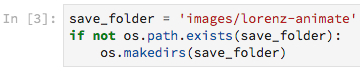
\includegraphics[width=8cm]{Input3A}
        \caption{Generamos una carpeta para organizar las imágenes.}
        \label{fig11:CarpetaA}
	\end{center}
\end{figure}

\vfill
\vline
\space
\par \vspace{4cm}

Nuestro cuarto bloque incluye los parámetros/valores iniciales que serán asignados a nuestro sistema.

\begin{figure}[h!]
	\begin{center}
		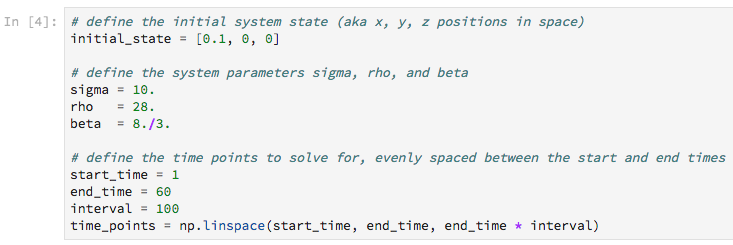
\includegraphics[width=13cm]{Input4A}
        \caption{Le asignamos los parámetros/valores iniciales al sistema.}
        \label{fig12:ValoresA}
	\end{center}
\end{figure}

Es momento de definir el sistema de Lorenz, el cual está conformado por tres EDO.

\begin{figure}[h!]
	\begin{center}
		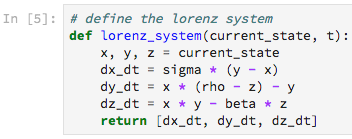
\includegraphics[width=6cm]{Input5A}
        \caption{Se define el sistema de Lorenz.}
        \label{fig13:DefinirA}
	\end{center}
\end{figure}

El siguiente paso consiste en crear las gráficas en planos tridimensionales. Es en este punto donde nosotros podemos establecer los límites a mostrar en nuestra gráfica en donde dice \textbf{ax.set\_xlim}, \textbf{ax.set\_ylim} y \textbf{ax.set\_zlim}, tal y como se muestra en la Figura \ref{fig14:GraficarA}. \\

\begin{figure}[h!]
	\begin{center}
		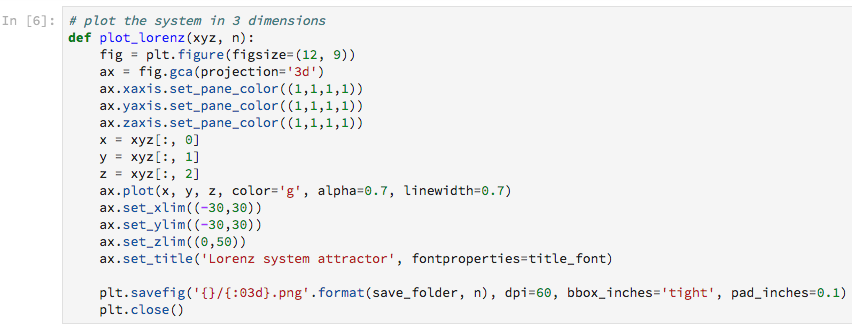
\includegraphics[width=15cm]{Input6A}
        \caption{Se gráfica el sistema en tres dimensiones.}
        \label{fig14:GraficarA}
	\end{center}
\end{figure}

Los siguientes tres bloques de código los presentaré a continuación en la Figura \ref{fig15:TresBloques}. En el último de ellos, el bloque 9, se adquieren los puntos a graficar, por lo cual este proceso puede tomar más tiempo que los anteriores.

\begin{figure}[h!]
	\begin{center}
		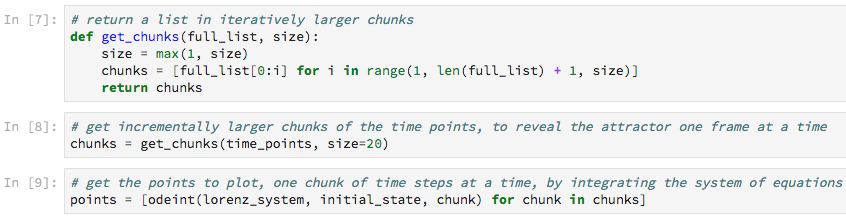
\includegraphics[width=16cm]{Input7-9A}
        \caption{En el bloque 9 se obtienen los puntos a graficar.}
        \label{fig15:TresBloques}
	\end{center}
\end{figure}

\vfill
\vline
\space
\par \vspace{1cm}

El siguiente de los pasos consiste en generar nuevamente las gráficas y guardar cada una de ellas en la carpeta \textbf{Lorenz-Animate} para utilizarlas posteriormente. Este paso es el que más tiempo tomará de todos los bloques de código del programa pues serán 300 imágenes (000 - 299.png) y el código se muestra en la Figura \ref{fig16:GuardarImagen}. \\

\begin{figure}[h!]
	\begin{center}
		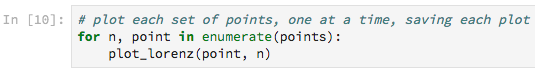
\includegraphics[width=14cm]{Input10A}
        \caption{Se generan y salvan las imágenes.}
        \label{fig16:GuardarImagen}
	\end{center}
\end{figure}

Ahora en los siguientes tres bloques de código se comienza a generar el archivo GIF. Primero se organizan todas las imágenes por utilizar, después el programa solicita que se carguen los archivos en el orden establecido, se procesan y salva el GIF. Todo esto se muestra en la Figura \ref{fig17:CompilaGIF}. \\

\begin{figure}[h!]
	\begin{center}
		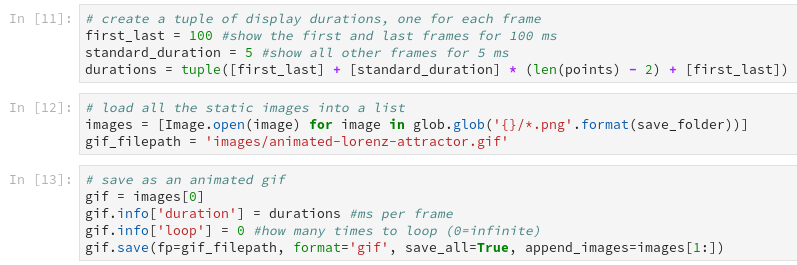
\includegraphics[width=16cm]{Input11-13A}
        \caption{Se crea el archivo GIF y se guarda.}
        \label{fig17:CompilaGIF}
	\end{center}
\end{figure}

Nuestro próximo bloque de código es simplemente para verifica el número de cuadros en el .GIF y el de imágenes que se habían generado inicialmente.

\begin{figure}[h!]
	\begin{center}
		\includegraphics[width=16cm]{Input14A}
        \caption{Verificamos el número de cuadros.}
        \label{fig18:VerificaCuadros}
	\end{center}
\end{figure}

\vfill
\vline
\space
\par \vspace{2cm}

Por último, mostramos el .GIF generado en nuestro programa haciendo uso del siguiente código.

\begin{figure}[h!]
	\begin{center}
		\includegraphics[width=16cm]{Input15A}
        \caption{Mostramos el .GIF en el programa.}
        \label{fig19:GeneraGIFCodigo}
        
        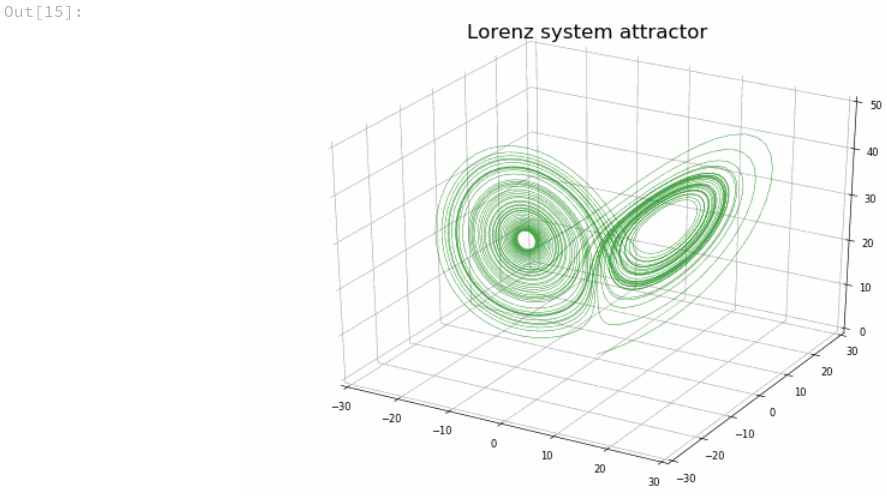
\includegraphics[height=9cm]{Output15A}
        \caption{Producto final generado.}
        \label{fig20:FinalGIF}
        
	\end{center}
\end{figure}

\vfill
\vline
\space
\par \vspace{2cm}

\section{Gráficas Bidimensionales}
Otro requisito en la actividad es generar tres gráficas bidimensionales que correspondan a cada uno de los ejes (x, y \& z) con respecto al tiempo.

Para llevar a cabo este requisito es necesario añadir un último código de bloque más al programa de \textsl{Visualización} para así poder usar los datos generados anteriormente y crear las tres gráficas o en una sola imagen graficar todo.

El código empleado para ello y el producto final se muestran en las Figuras \ref{fig21:3en1} y \ref{fig22:3en1Graf}, respectivamente.

\begin{figure}[h!]
	\begin{center}
		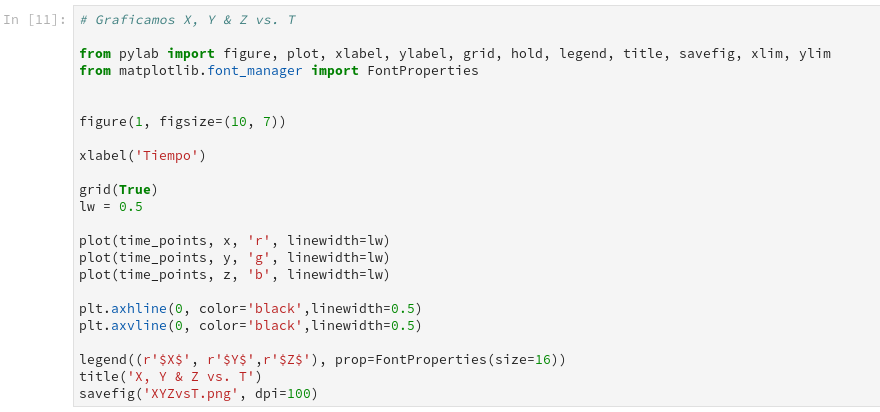
\includegraphics[width=15cm]{BiGrafCod-1}
        \caption{Generaremos los gráfico bidimensional.}
        \label{fig21:3en1}
        
        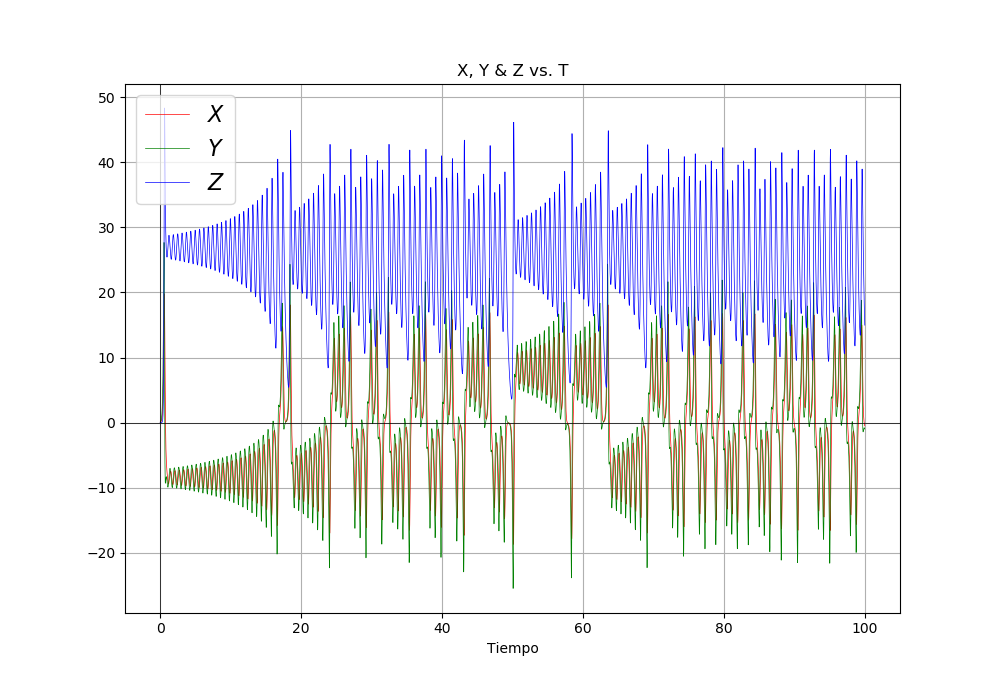
\includegraphics[width=15cm]{XYZvsT-1}
        \caption{Gráfica del sistema de EDO contra el tiempo.}
        \label{fig22:3en1Graf}
        
	\end{center}
\end{figure}

\section{Ajuste de parámetros}
En esta sección veremos cómo se ve alterado el sistema de Lorenz al modificar los parámetros $\sigma$, $\beta$ \& $\rho$ en bloque de código 4 de ambos programas (\textsl{Visualización} \& \textsl{Animación}).

\subsection{Primer cambio de parámetros}
Ahora nos dirigiremos al bloque número 4 en ambos programas y daremos nuevos valores a los parámetros, los cuales serán los siguientes:

\begin{center}
	$ Sigma ( \sigma ) = 28 $ \\
    $ Rho ( \rho ) = 46.92 $ \\
    $ Beta ( \beta ) = 4 $
\end{center}

El nuevo código genera las siguientes imágenes:

\begin{itemize}
\item \textbf{Atractor de Lorenz.}

Imagen correspondiente a la Figura \ref{fig23:PrimAjus-A}.

\begin{figure}[h!]
	\begin{center}
		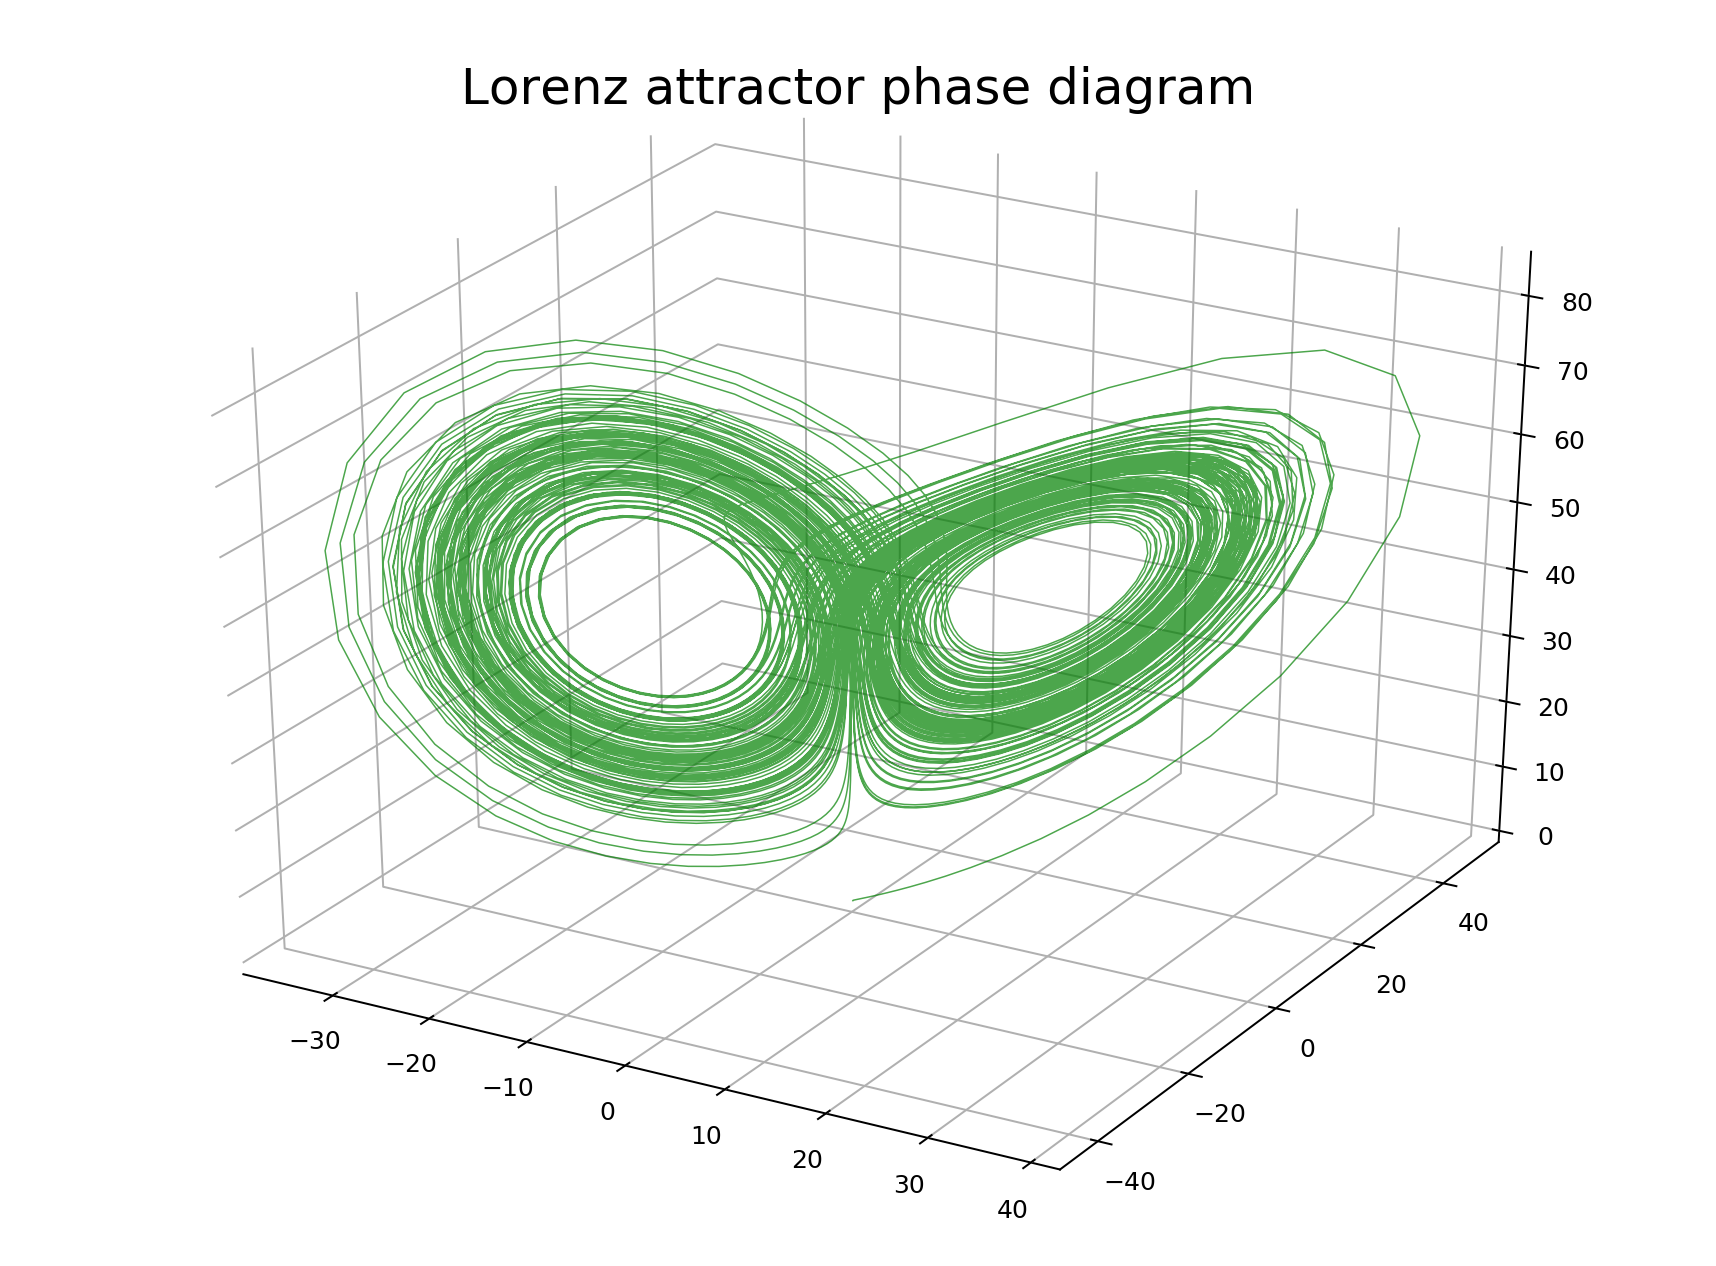
\includegraphics[width=13cm]{AtractorLorenz3D-2}
        \caption{Primer ajuste de parámetros en el atractor 3D.}
        \label{fig23:PrimAjus-A}
	\end{center}
\end{figure}

\item \textbf{Gráficas entre los planos.}

Imagen correspondiente a la Figura \ref{fig24:PrimAjus-B}.

\begin{figure}[h!]
	\begin{center}
		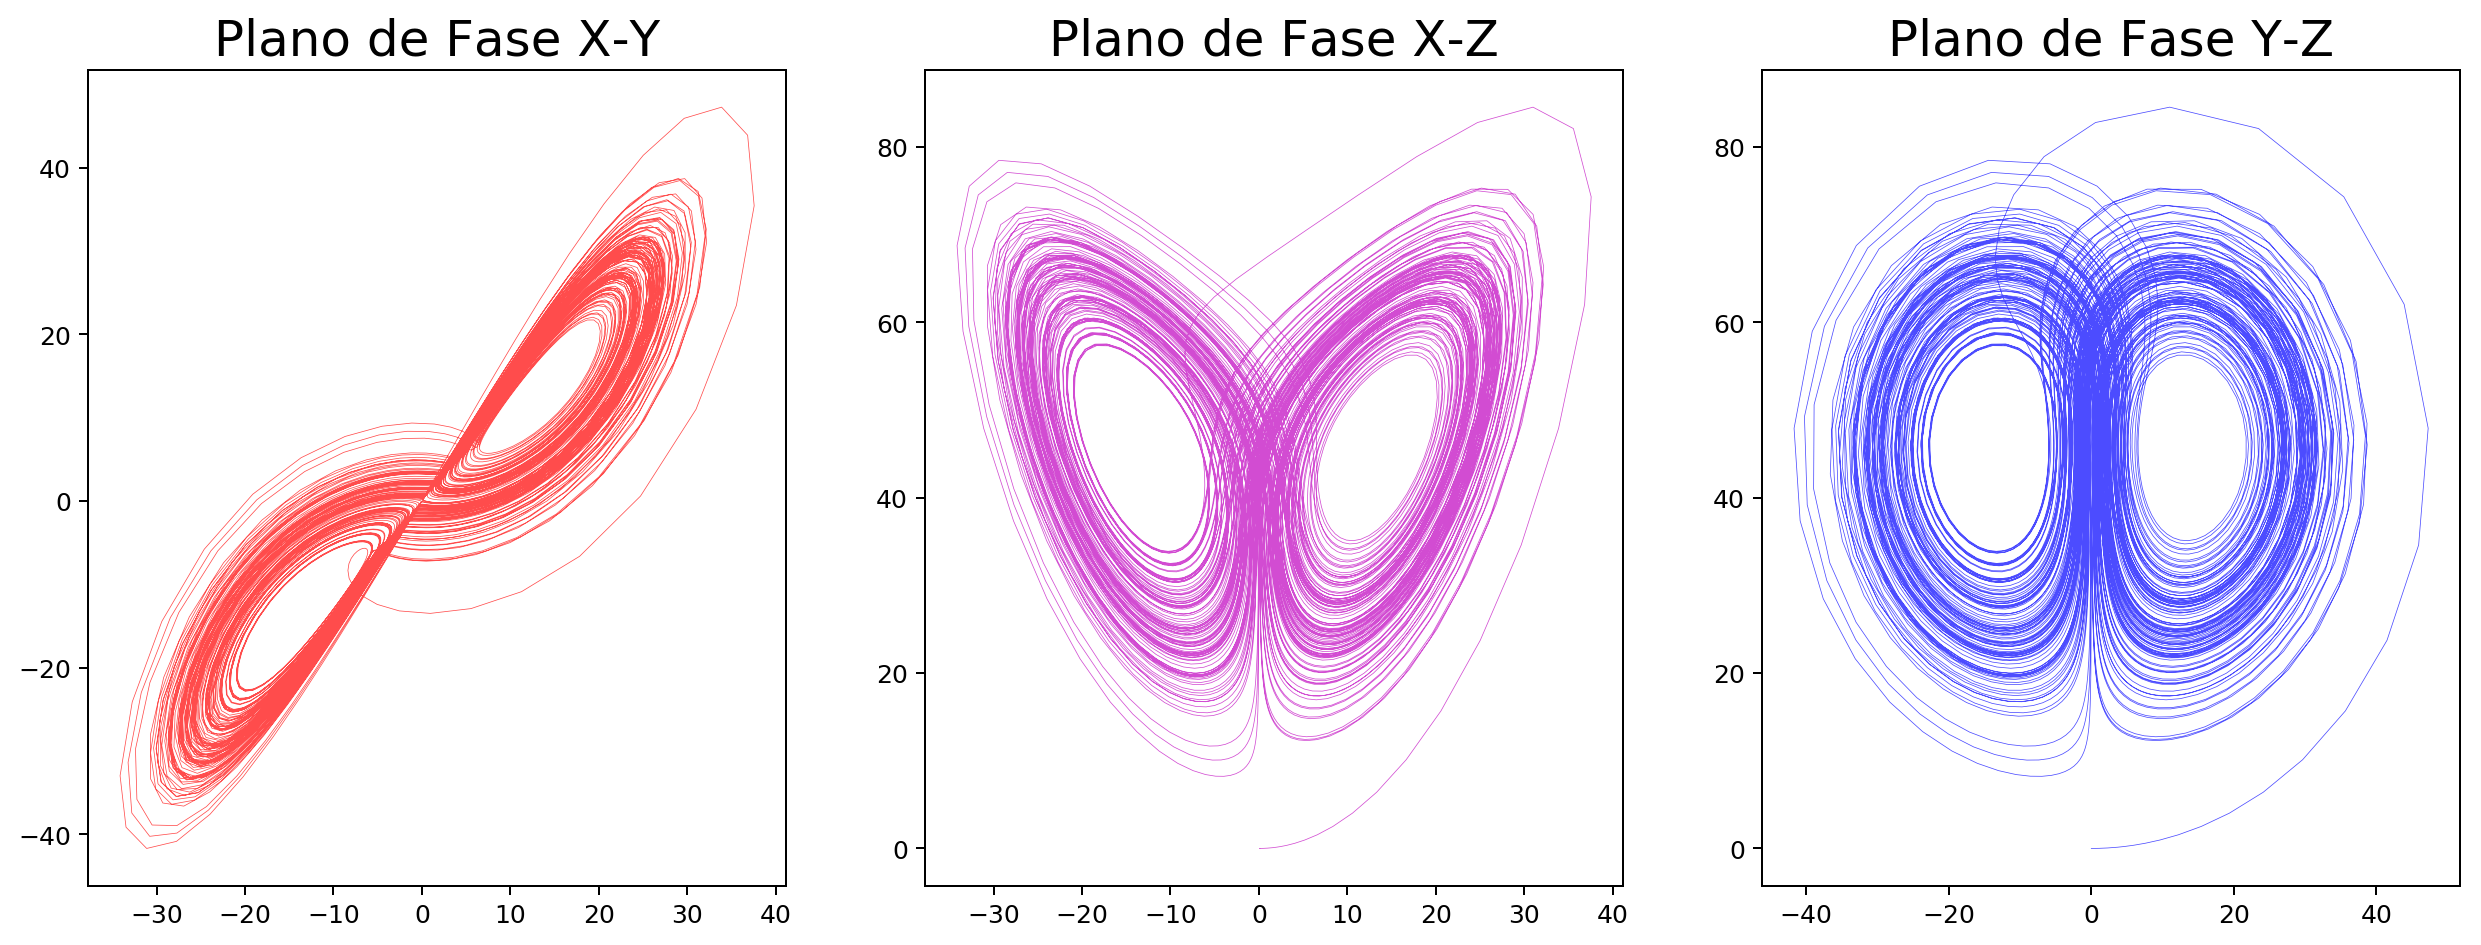
\includegraphics[width=15cm]{AtractorLorenzXYZ-2}
        \caption{Primer ajuste de parámetros en el atractor en planos.}
        \label{fig24:PrimAjus-B}
	\end{center}
\end{figure}

\item \textbf{Gráfica de los ejes con respecto al tiempo.}

Imagen correspondiente a la Figura \ref{fig25:PrimAjus-C}

\begin{figure}[h!]
	\begin{center}
		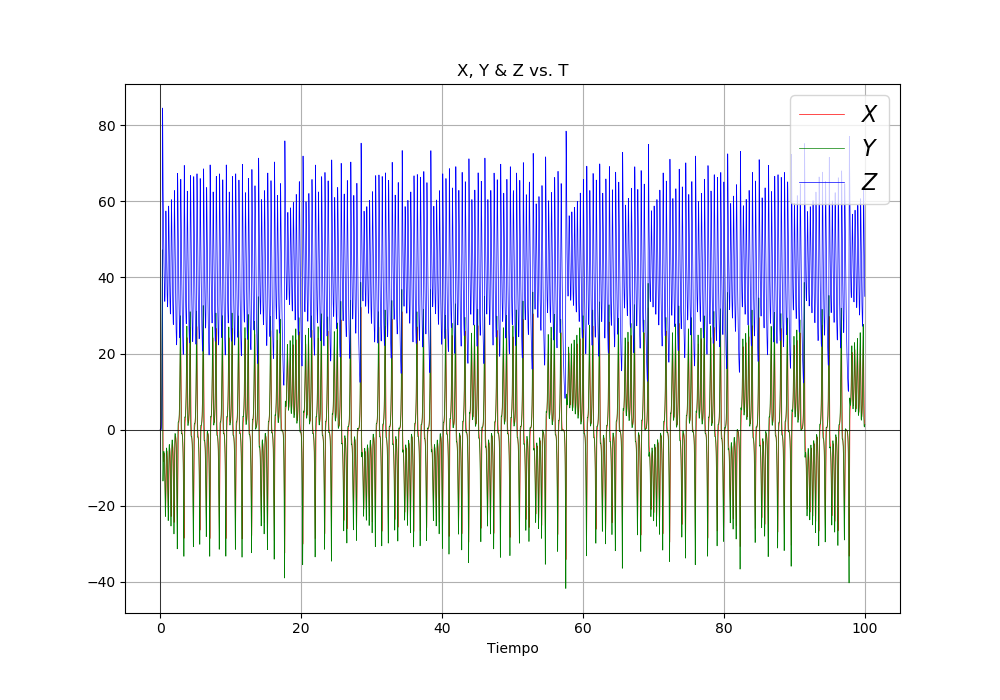
\includegraphics[width=13cm]{XYZvsT-2}
        \caption{Primer ajuste de parámetros en el atractor en ejes contra tiempo.}
        \label{fig25:PrimAjus-C}
	\end{center}
\end{figure}

\end{itemize}

\subsection{Segundo cambio de parámetros}

De igual manera que en el primero, en nuestro bloque de código 4 de nuestros programas hemos de modificar los parámetros señalados, dándole los siguientes nuevos valores:

\begin{center}
	$ Sigma ( \sigma ) = 10 $ \\
    $ Rho ( \rho ) = 99.96 $ \\
    $ Beta ( \beta ) = \dfrac{8}{3} $
\end{center}

De igual forma, la alteración de dichos parámetros nos genera:

\begin{itemize}
\item \textbf{Atractor de Lorenz.}

Imagen correspondiente a la Figura \ref{fig26:SeguAjus-A}.

\begin{figure}[h!]
	\begin{center}
		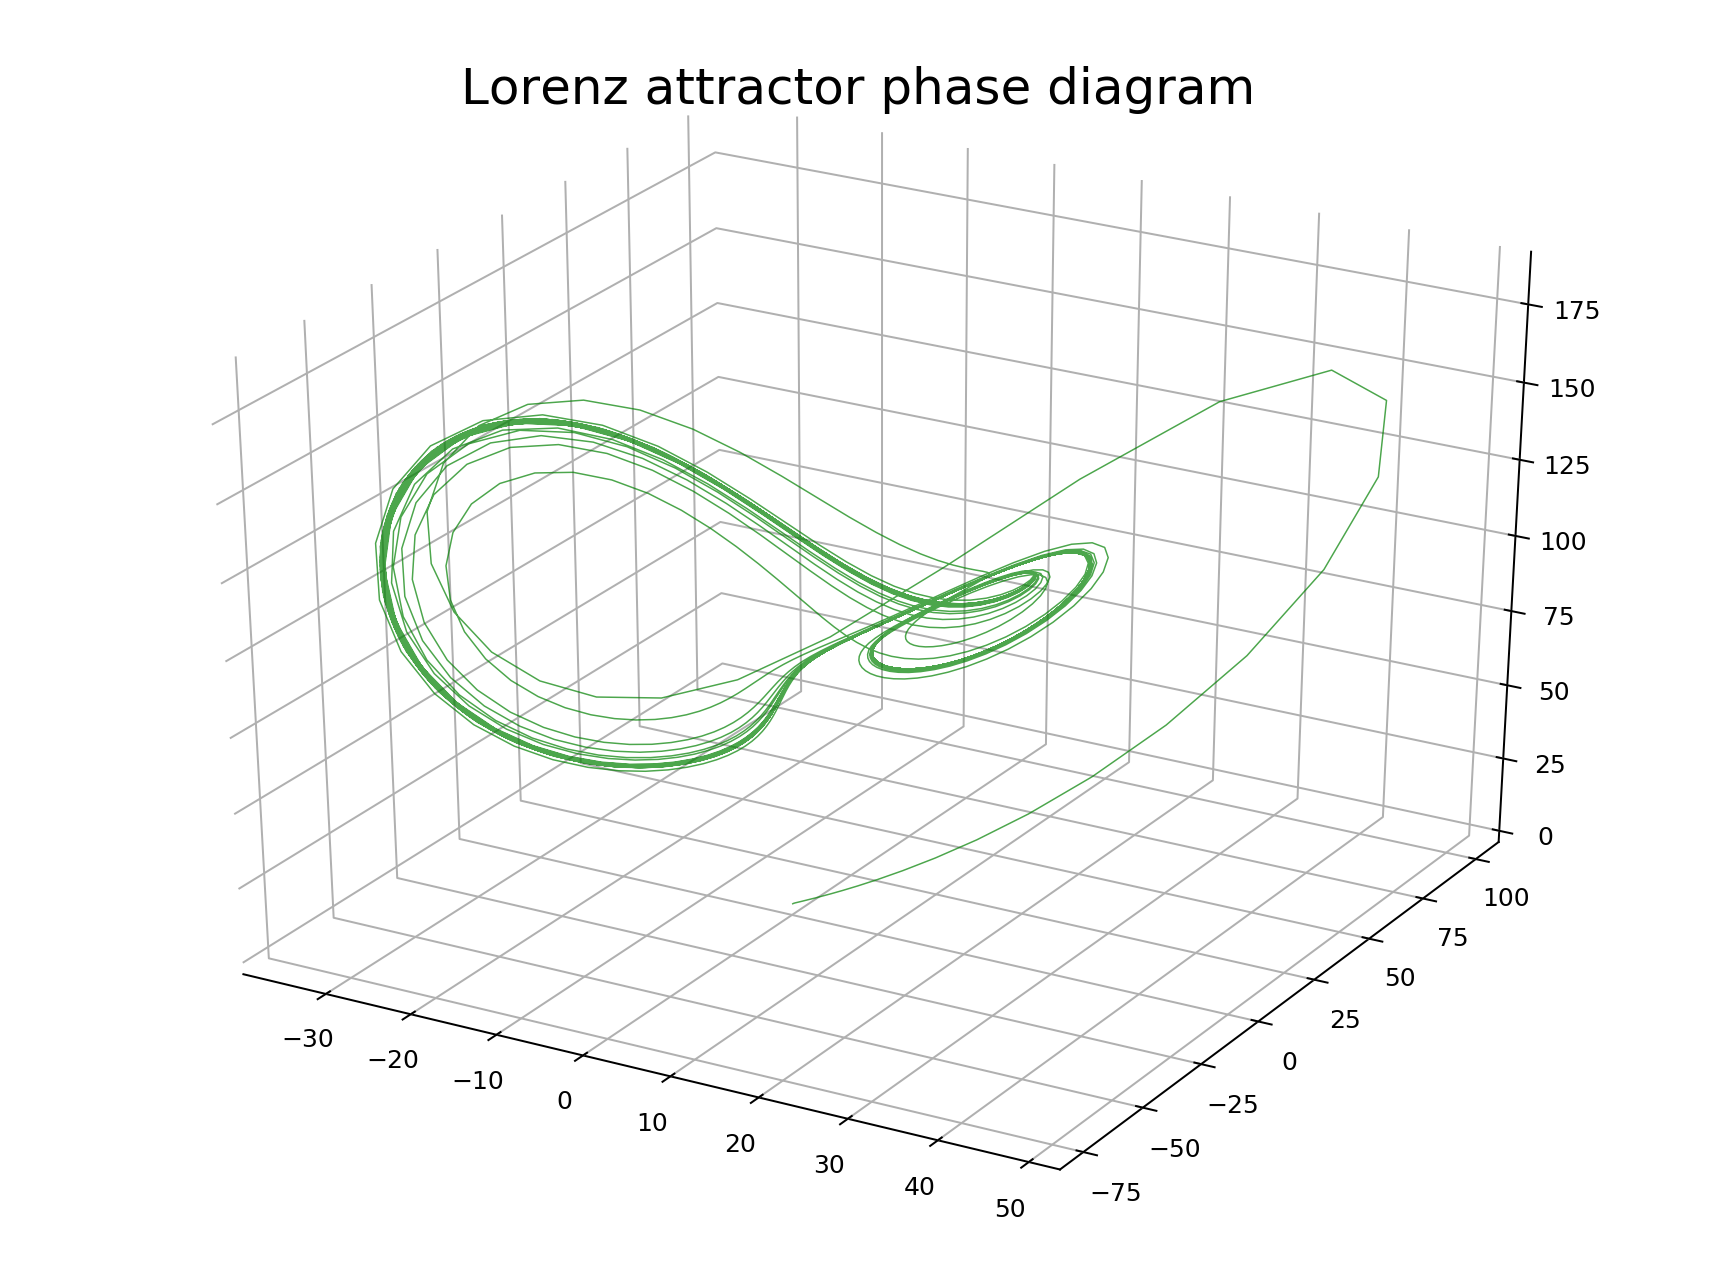
\includegraphics[width=13cm]{AtractorLorenz3D-3}
        \caption{Segundo ajuste de parámetros en el atractor 3D.}
        \label{fig26:SeguAjus-A}
	\end{center}
\end{figure}

\item \textbf{Gráficas entre los planos.}

Imagen correspondiente a la Figura \ref{fig27:SeguAjus-B}.

\begin{figure}[h!]
	\begin{center}
		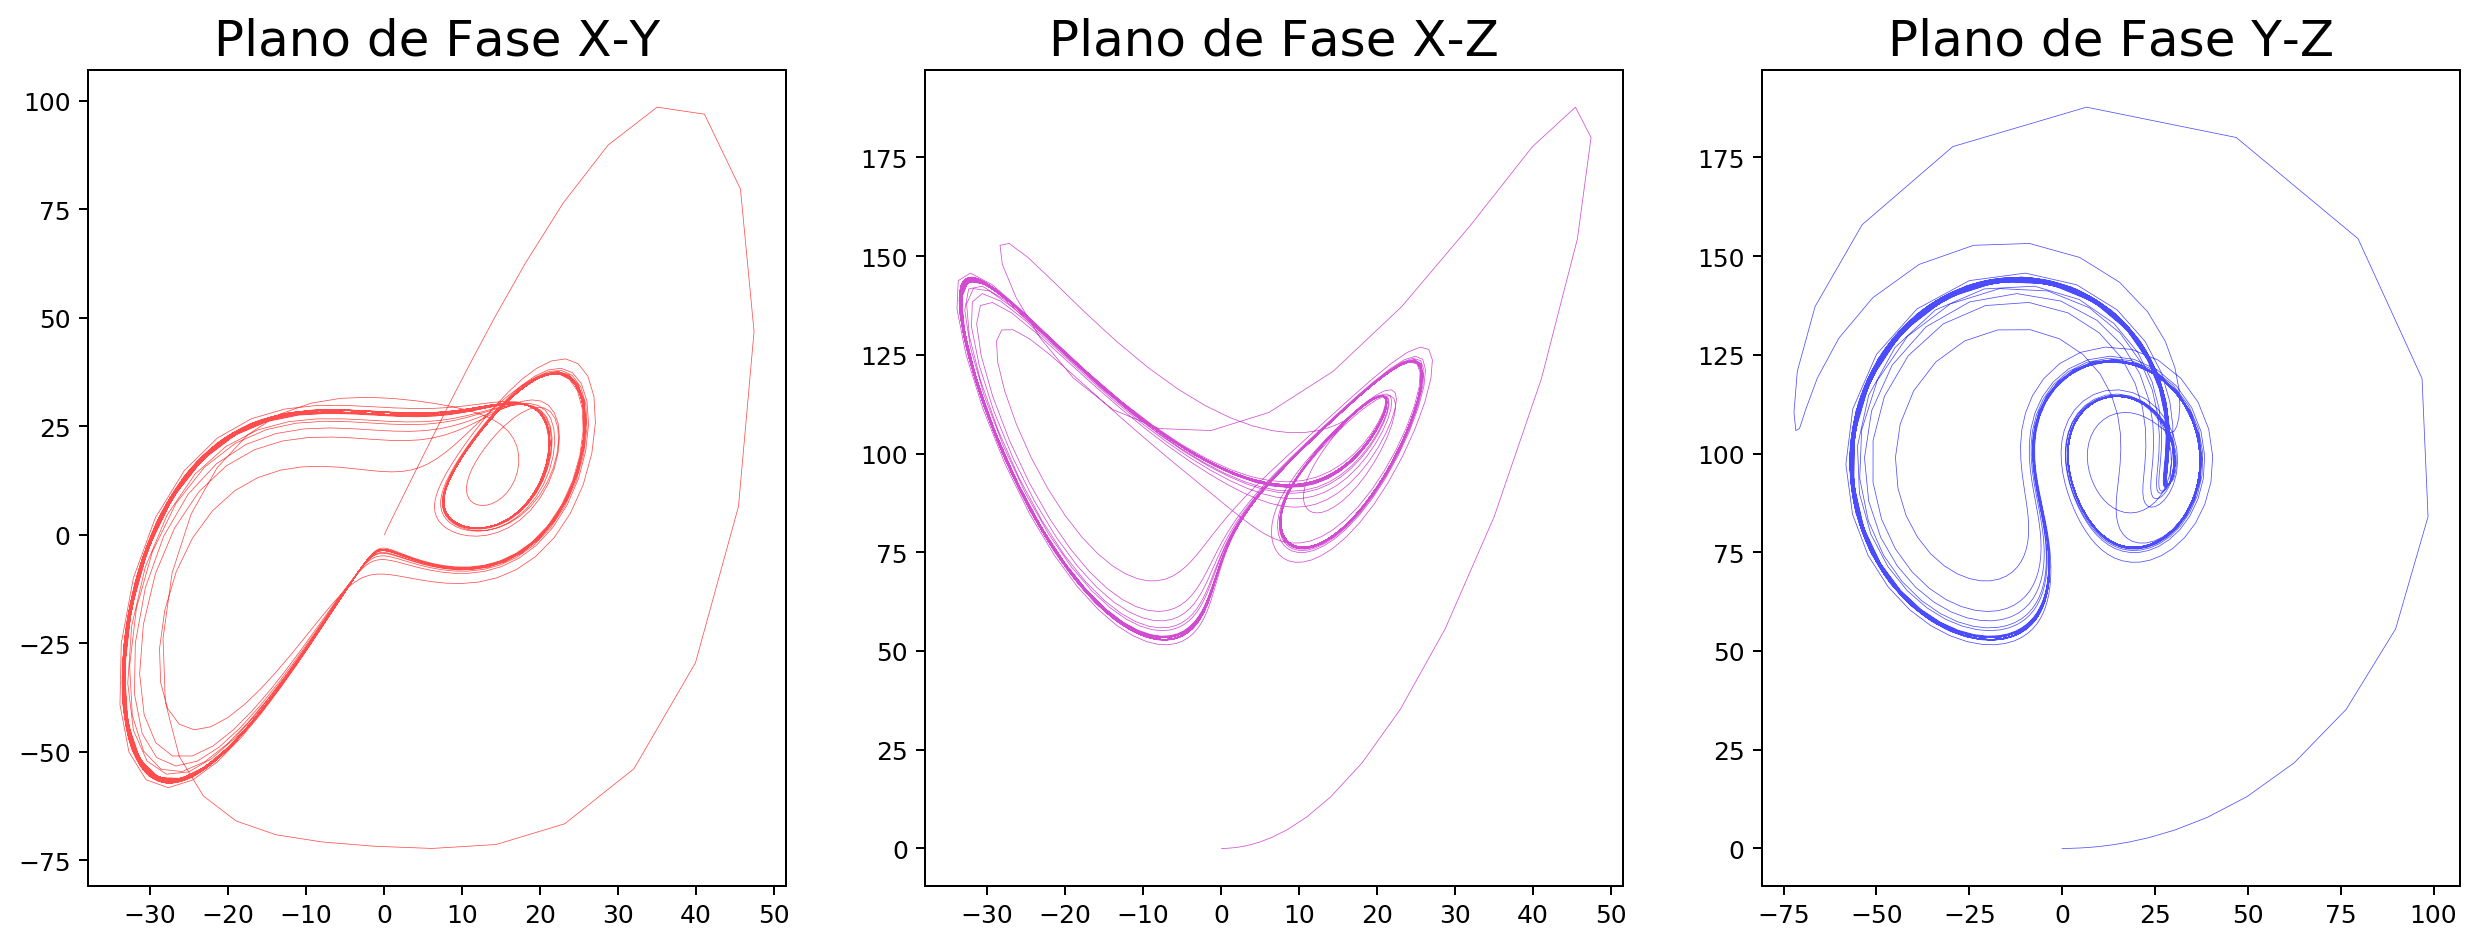
\includegraphics[width=14cm]{AtractorLorenzXYZ-3}
        \caption{Segundo ajuste de parámetros en el atractor en planos.}
        \label{fig27:SeguAjus-B}
	\end{center}
\end{figure}

\item \textbf{Gráfica de los ejes con respecto al tiempo.}

Imagen correspondiente a la Figura \ref{fig28:SeguAjus-C}.

\begin{figure}[h!]
	\begin{center}
		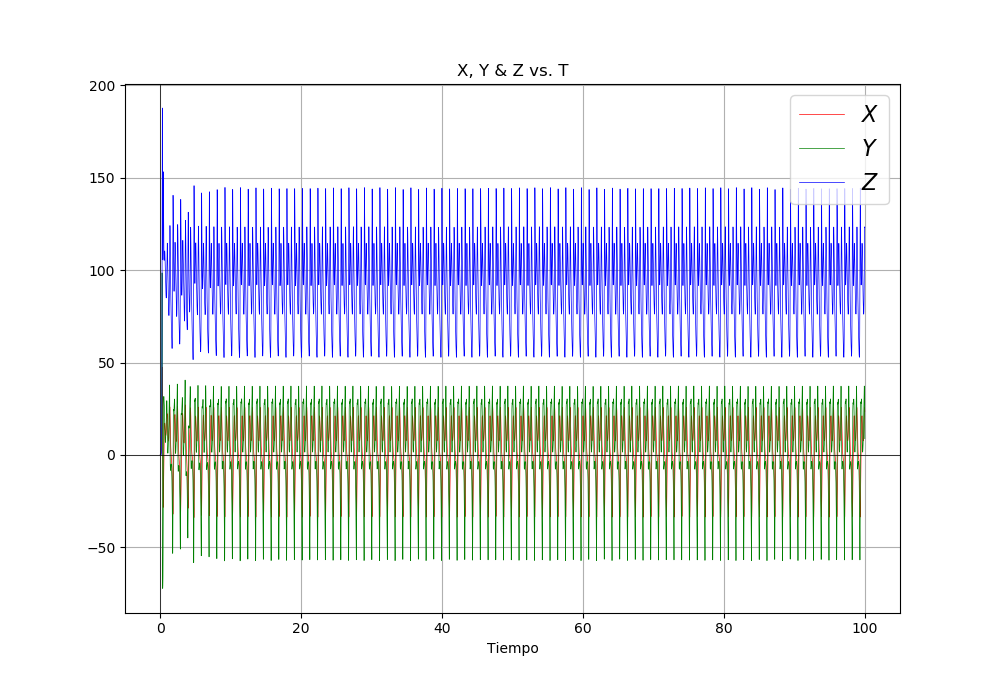
\includegraphics[width=14cm]{XYZvsT-3}
        \caption{Segundo ajuste de parámetros en el atractor en ejes contra tiempo.}
        \label{fig28:SeguAjus-C}
	\end{center}
\end{figure}

\end{itemize}

\section{Conclusión}

Si hacemos una comparación entre todas las gráficas generadas podremos apreciar cómo es que cambia el comportamiento del sistema de Lorenz en base a los parámetros dados, siendo este un sistema muy sensible a dichos valores.

\end{document}